\documentclass{article}
\usepackage{graphicx}
\usepackage{amsmath} 

\title{\textbf{Theoretical Questions Chapter 4}}
\author{Ling Siu Hong \\ 3200300602}
\begin{document}
\maketitle

\textbf{A} : The following result be
    \begin{center}
		  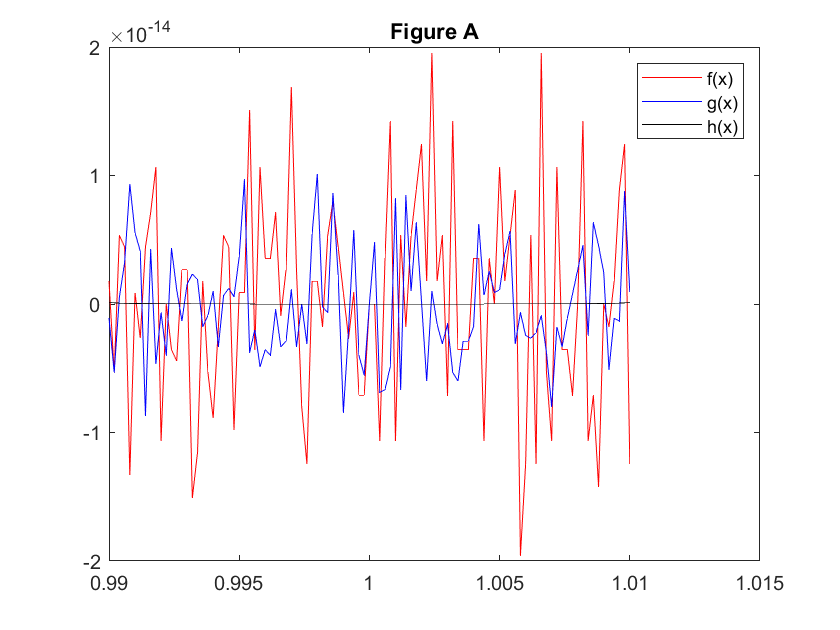
\includegraphics[width=11cm]{Picture A.png}	
    \end{center}.
    The $f(x)$ has the most obviously oscillation,which means that it is unstable.This is because of more calculation is doing leads to more round off.The $g(x)$ has smaller amplitude due to less calculation are doing.It is obvious that $h(x)$ has the least number of calculation,therefore it is most accurate.

\textbf{B} : 
\begin{itemize}
    \item UFL = 0.5 and OFL = 3.5
    \item Cardinality of $#\mathcal{F} =  25$ 
    Normal number in $\mathcal{F}$ :
    -3.5 , -3 , -2.5 , -2 , -1.75 , -1.5 , -1.25 , -1 , -0.875 , -0.75 , -0.625 , -0.5 , 0 , 0.5 , 0.625 , 0.75 , 0.875 , 1 , 1.25 , 1.5 , 1.75 , 2 , 2.5 , 3 , 3.5 
        \begin{center}
		  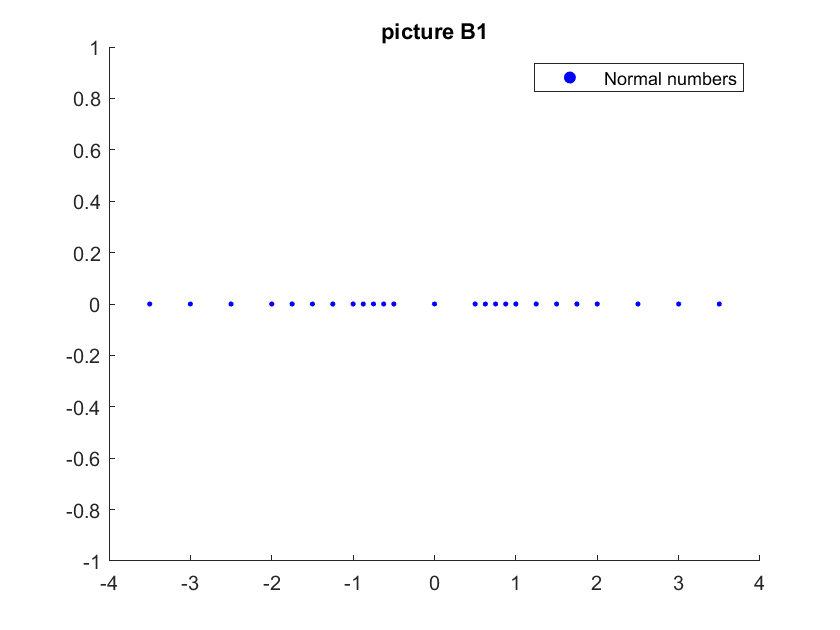
\includegraphics[width=11cm]{Picture B1.png}	
        \end{center}
    \item Subnormal number in $\mathcal{F}$ :
    -0.1875, -0.125, -0.0625, 0.0625, 0.125, 0.1875

        \begin{center}
		  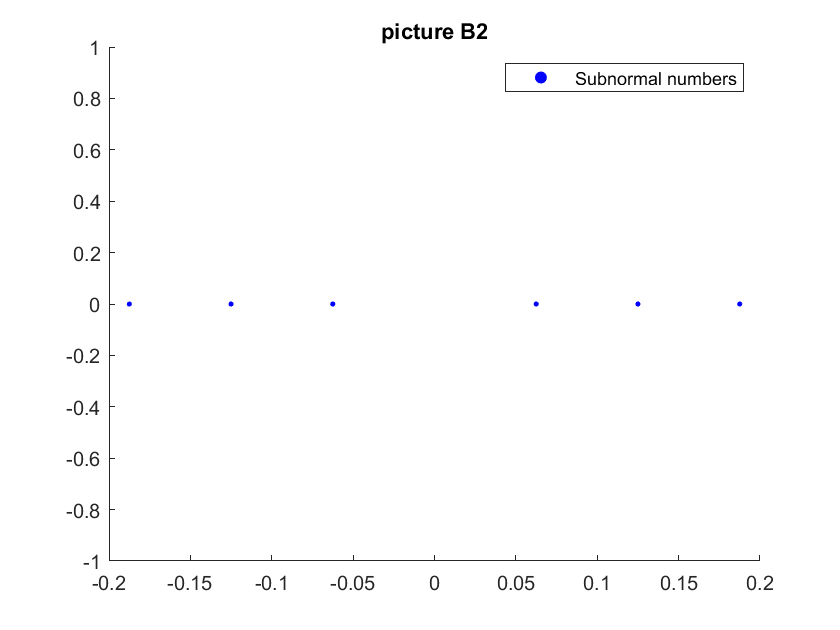
\includegraphics[width=11cm]{Picture B2.png}	
        \end{center}
\end{itemize}
\end{document}